\documentclass{beamer}

\usepackage[utf8]{inputenc}
\usepackage[portuguese]{babel}

\usetheme{JuanLesPins}

\title{TCC 1}
\subtitle{PROCESSAMENTO DE DADOS EM UMA PLATAFORMA DE CIDADES INTELIGENTES}
\author{Dylan Guedes}
\institute{UnB Gama}
\date{\today}

\begin{document}
  \begin{frame}
    \titlepage
    Orientador: Prof. Dr. Paulo Roberto Miranda Meirelles
    Co-orientador: Arthur de Moura Del Esposte
\end{frame}

  \begin{frame}
    \frametitle{Cidades inteligentes}

    \begin{itemize}
        \item \textbf{Cidades inteligentes} podem ser definidas como a
            utilização de tecnologias da informação e comunicação para
            melhorar a vida da população;

        \item \textbf{Plataformas de cidades inteligentes} ajudam aplicações
            a serem desenvolvidas, fornecendo serviços;
    \end{itemize}
\end{frame}

  \begin{frame}
    \frametitle{Iniciativas ocorrendo}
    \begin{itemize}
        \item Na Espanha, a plataforma \textbf{SmartSantander} é utilizada
            por diversas aplicações de cidades inteligentes;

        \begin{figure}
            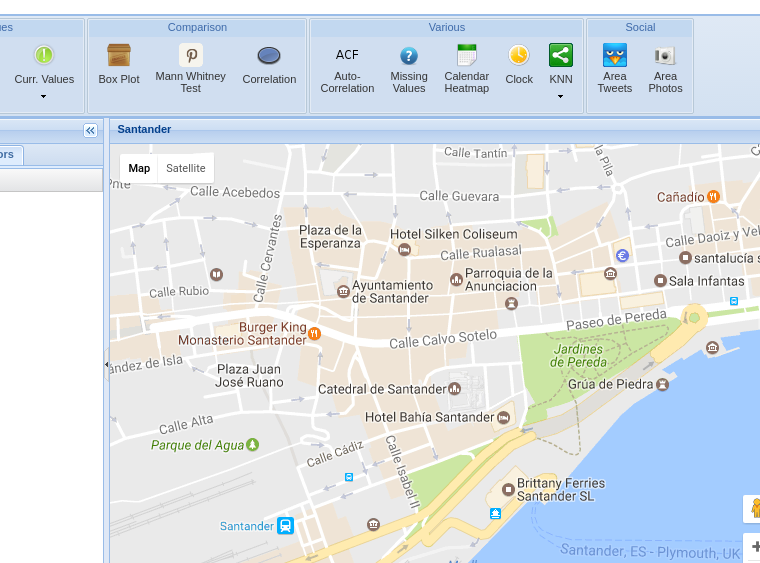
\includegraphics[scale=0.2]{figures/sen2soc.png}
            \caption{Aplicativo Sen2Soc, que utiliza o SmartSantander.}
        \end{figure}
    \end{itemize}
\end{frame}

  \begin{frame}
    \frametitle{Iniciativas ocorrendo}
    \begin{itemize}
        \item Na Holanda, através da plataforma \textbf{Amsterdam Smart City},
            aplicações de cidades inteligentes são divulgadas.

        \begin{figure}
            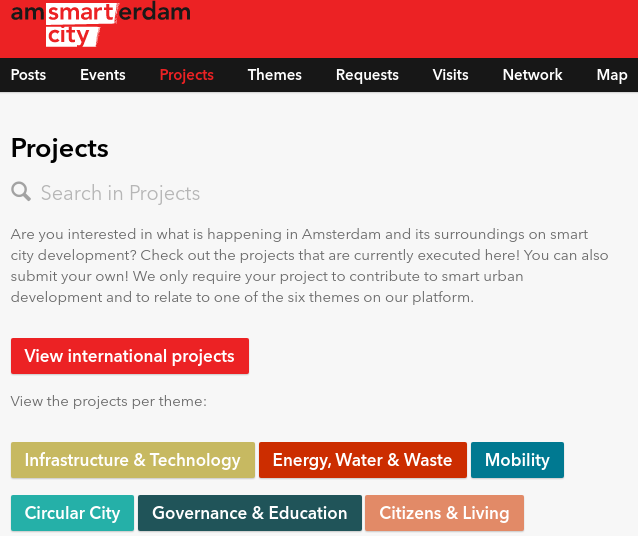
\includegraphics[scale=0.25]{figures/asc.png}
            \caption{Plataforma Amsterdam Smart City (ASC).}
        \end{figure}
    \end{itemize}
\end{frame}

  \begin{frame}
    \frametitle{Problemas nas soluções atuais}
    \begin{itemize}
        \item Desafios técnicos continuam em aberto;
        \item Soluções específicas, não promovem a interoperabilidade.
    \end{itemize}
\end{frame}

  \begin{frame}
    \frametitle{Surgimento do InterSCity}
    \begin{itemize}
        \item Plataforma que se preocupe com os problemas de interoperabilidade;
        \item Suporte ao desenvolvimento de aplicações de cidades inteligentes;
        \item Arquitetura baseada em microsserviços.
    \end{itemize}
\end{frame}

  \begin{frame}
    \frametitle{Características do InterSCity}
    \begin{itemize}
        \item Licenciado sob MPLv2;
        \item Arquitetura de microsserviços (MSA);
        \item Maior parte em Ruby on Rails
    \end{itemize}
\end{frame}

  \begin{frame}
    \frametitle{Arquitetura do InterSCity}
    \begin{itemize}
        \item Microsserviços conversam utilizando REST e passagem de mensagem;
        \item Passagem de mensagem feita com RabbitMQ.
            \begin{figure}
                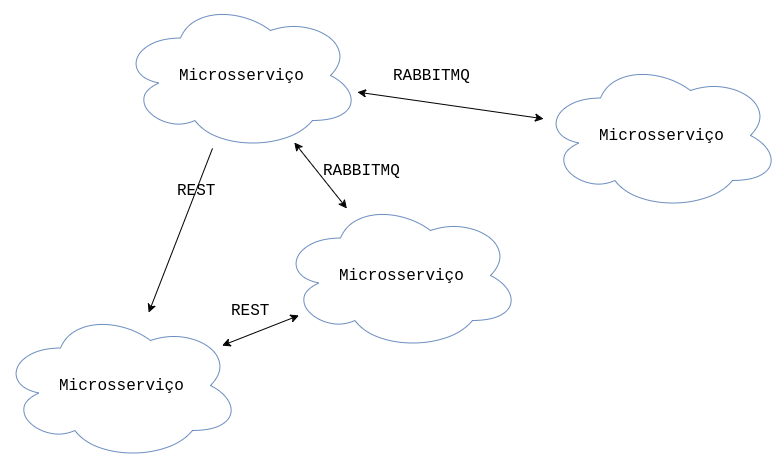
\includegraphics[scale=0.3]{figures/communication.png}
                \caption{Comunicação utilizando REST e passagem de mensagem.}
            \end{figure}
    \end{itemize}
\end{frame}

  \begin{frame}
    \frametitle{Arquitetura do InterSCity}
    \begin{itemize}
        \item
            \begin{figure}
                \includegraphics[scale=0.3]{figures/interscity_architecture.png}
                \caption{Microsserviços e arquitetura do InterSCity.}
            \end{figure}
    \end{itemize}
\end{frame}

  \begin{frame}
    \frametitle{Processamento de Dados}
    \begin{itemize}
        \item Cidades inteligentes precisam dos três V's para certos cenários:
            \begin{itemize}
                \item Volume
                \item Velocidade
                \item Variedade
            \end{itemize}
    \end{itemize}
\end{frame}

  \begin{frame}
    \frametitle{Ferramenta chave - Big Data}
    \begin{itemize}
        \item Ferramentas específicas para cenários de larga escala de dados.
        \item Análise de dois padrões de projeto - Arquitetura Lambda e Arquitetura Kappa.
    \end{itemize}
\end{frame}

\begin{frame}
    \frametitle{Arquitetura Lambda}
    \begin{itemize}
        \item Separação em camadas \textbf{\textit{streaming}} e
            \textbf{\textit{batch}};
        \item Camada \textit{batch} faz o processamento a todo o tempo, mas
            apresenta alta latência;
        \item Camada \textit{speed} faz o processamento como complemento aos
            dados não levados em conta pela \textit{batch};
        \item Soma entre os resultados das duas camadas.
    \end{itemize}
\end{frame}


  \begin{frame}
      \frametitle{Arquitetura Kappa}
      \begin{figure}
          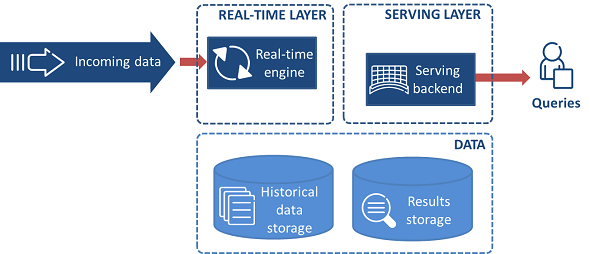
\includegraphics[scale=0.4]{figures/KappaArchitecture.png}
          \caption{Arquitetura Kappa. Fonte: Sony Ericsson.}
      \end{figure}
      \begin{itemize}
          \item Utiliza somente processamento \textit{streaming}.
          \item Utiliza a retenção do log para uso de dados históricos.
          \item Baixa latência.
      \end{itemize}
  \end{frame}
  
  \begin{frame}
      \frametitle{Lambda vs Kappa}
      \begin{itemize}
          \item Lambda é mais complexa.
          \item Kappa não pode ser utilizada em certos contextos.
      \end{itemize}
  \end{frame}

  \begin{frame}
      \frametitle{Análise de Ferramentas}
      \begin{itemize}
          \item Análise de ferramentas de processamento streaming e batch.
          \item Análise de broker.
      \end{itemize}
  \end{frame}

  \begin{frame}
      \frametitle{Processamento batch - MapReduce vs Spark}
      \begin{figure}
          
\includegraphics[scale=0.3]{figures/BatchProcessing.png}
      \end{figure}
      \begin{itemize}
          \item MapReduce permite uso de qualquer linguagem que possua interação
              com I/O padrão.
          \item Spark apresenta latência bem menor que o MapReduce.
          \item Spark dispõe de biblioteca de ML.
          \item Spark pode ser usado como processamento \textit{streaming}.
      \end{itemize}
  \end{frame}

  \begin{frame}
      \frametitle{Processamento streaming - Spark vs Storm}
      \begin{figure}
          
\includegraphics[scale=0.6]{figures/StreamingProcessing.png}
      \end{figure}
      \begin{itemize}
          \item Storm apresenta menor latência que o Spark.
          \item Storm pode ser utilizando com qualquer linguagem que possua
              interação com I/O padrão.
          \item Abordagens diferentes - Spark usa \textit{micro-batch}, Storm utiliza
              \textit{streaming}.
          \item Spark pode ser usado para processamento \textit{batch}.
          \item Spark dispõe de biblioteca de ML.
      \end{itemize}
  \end{frame}

  \begin{frame}
      \frametitle{Broker - Kafka vs RabbitMQ}
      \begin{figure}
          
\includegraphics[scale=0.3]{figures/Brokers.png}
      \end{figure}
      \begin{itemize}
          \item RabbitMQ já é utilizado pelo InterSCity.
          \item RabbitMQ dispõe de \textit{plugins} para estender as funcionalidades.
          \item RabbitMQ permite a utilização de filas e tópicos mais complexos.
          \item Kafka apresenta performance superior.
          \item Kafka tem integração nativa com o Spark.
          \item Kafka armazena o \textit{log}.
      \end{itemize}
  \end{frame}

  \begin{frame}
      \frametitle{Novo serviço de processamento}
      \begin{itemize}
          \item<2-> Utilização da \textbf{Arquitetura Kappa}.
          \item<3-> \textbf{Apache Spark} para processamento \textit{streaming};
          \item<4-> \textbf{Apache Kafka} como \textit{broker}.
      \end{itemize}
  \end{frame}

  \begin{frame}
      \frametitle{Arquitetura Kappa}
      \begin{figure}
          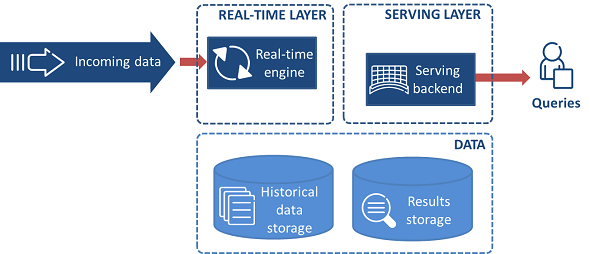
\includegraphics[scale=0.4]{figures/KappaArchitecture.png}
      \end{figure}
      \begin{itemize}
          \item Complexidade da Arquitetura Lambda.
          \item Melhor adoção para o time do InterSCity.
      \end{itemize}
  \end{frame}

  \begin{frame}
      \frametitle{Apache Spark}
      \begin{itemize}
          \item Biblioteca de ML nativa;
          \item Poder utilizar Python;
          \item Fácil troca para a Arquitetura Lambda.
              \begin{figure}
                  
\includegraphics[scale=0.3]{figures/spark_logo.png}
              \end{figure}
      \end{itemize}
  \end{frame}

  \begin{frame}
      \frametitle{Apache Kafka}
      \begin{itemize}
          \item Ajuda na implementação da Arquitetura Kappa;
          \item Produtor nativo para o Spark Streaming;
          \item Utilização somente no processamento de dados.
              \begin{figure}
                  
\includegraphics[scale=0.3]{figures/kafka_logo.png}
              \end{figure}
      \end{itemize}
  \end{frame}

  \begin{frame}
      \frametitle{Implementação}
      \begin{itemize}
          \item Divisão em três etapas:
              \begin{itemize}
                  \item Configuração do ambiente;
                  \item Interoperabilidade entre os serviços;
                  \item Possibilidade de estender o processamento de uma forma customizável.
              \end{itemize}
      \end{itemize}
  \end{frame}

  \begin{frame}
      \frametitle{Shock}
      \begin{itemize}
          \item Aplicação que abstrai o uso do Spark e do Kafka;
          \item Faz parte do novo serviço de processamento de dados;
          \item Carrega novas operações para o pipeline de dados via Kafka;
      \end{itemize}
  \end{frame}

  \begin{frame}
      \frametitle{Ciclo básico do Shock}
          \begin{figure}
              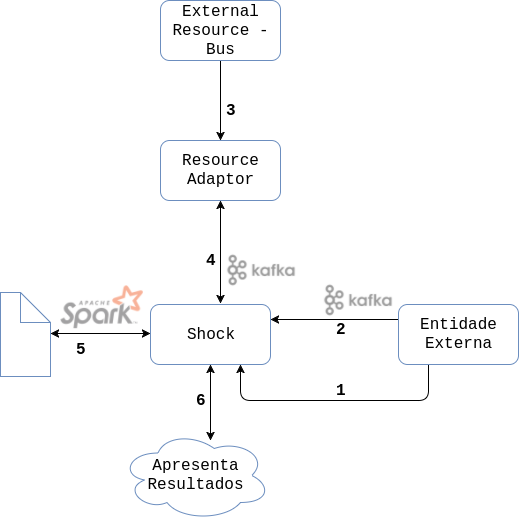
\includegraphics[scale=0.3]{figures/shock.png}
          \end{figure}
  \end{frame}

  \begin{frame}
      \frametitle{Contribuições}
      \begin{itemize}
          \item Novo serviço de processamento
          \item Aplicação que abstrai outras ferramentas, e que é extensível
          \item Possibilidade de uso de algoritmos sofisticados
          \item Possibilidade de atuação em cenários mais extremos
      \end{itemize}
  \end{frame}

  \begin{frame}
      \frametitle{Próximos passos - TCC 2}
      \begin{itemize}
          \item Segunda rodada de revisão na bibliografia.
          \item Desacoplar o núcleo do Shock do Kafka.
          \item Testar o núcleo do Shock.
          \item Documentar a API de serviços.
          \item Disponibilizar customização de janelas de micro-batch.
          \item Utilizar recuperação de dados históricos através dos logs do Kafka.
      \end{itemize}
  \end{frame}

  \begin{frame}
      \frametitle{Próximos passos - Após o TCC 2}
      \begin{itemize}
          \item Utilizar outras estruturas de dados (não só RDD's).
          \item Uso de check-points.
          \item Múltiplos streams.
      \end{itemize}
  \end{frame}
\end{document}
